\documentclass[10pt]{article}

\usepackage{fancyhdr}
\usepackage[includeheadfoot,left=1in, right=0.5in, top=0.5in, bottom=0.5in]{geometry}
\usepackage{lastpage}
\usepackage{extramarks}
\usepackage[usenames,dvipsnames]{color}
\usepackage{graphicx}
\usepackage{listings}
\usepackage{courier}
\usepackage{float}
\usepackage{url}
\usepackage{subfigure}
\usepackage{varwidth}
\usepackage{caption}
\usepackage{multirow}
\usepackage[pdfborder={0 0 0}]{hyperref}
\usepackage[compact,small]{titlesec}
\usepackage{microtype}
\usepackage{verbatim}
\usepackage{booktabs}
\usepackage{indentfirst}
\usepackage{pgffor}
\usepackage{mathtools}
\usepackage{amsmath}
\usepackage[table]{xcolor}

\rowcolors{2}{gray!25}{white}

\parskip = 0.5\baselineskip
\setlength{\belowcaptionskip}{-\baselineskip}

\captionsetup{font=scriptsize}
\captionsetup{labelfont=bf}

\pagestyle{fancy}
\rhead{Max Thrun | Samir Silbak}
\lhead{EECE6086 - HW 3}
\rfoot{Page\ \thepage\ of \protect\pageref{LastPage}}
\cfoot{}
\renewcommand\headrulewidth{0.4pt}
\renewcommand\footrulewidth{0.4pt}

% make verbatim text small
\makeatletter
\g@addto@macro\@verbatim\tiny
\makeatother

\setlength\parindent{0pt} % Removes all indentation from paragraphs

\definecolor{sh_comment}{rgb}{0.12, 0.38, 0.18 } %adjusted, in Eclipse: {0.25, 0.42, 0.30 } = #3F6A4D
\definecolor{sh_keyword}{rgb}{0.37, 0.08, 0.25}  % #5F1441
\definecolor{sh_string}{rgb}{0.06, 0.10, 0.98} % #101AF9

\lstset{
    language=c++,
    xleftmargin=.25in,
    xrightmargin=.25in,
    numbers=left,
    numberstyle=\tiny,
    frame=tb,
    showstringspaces=false,
    captionpos=b,
    stringstyle=\color{sh_string},
    keywordstyle = \color{sh_keyword}\bfseries,
    commentstyle=\color{sh_comment}\itshape,
    basicstyle=\footnotesize\sffamily,
    %numbersep=-5pt,
    belowskip=\baselineskip,
    aboveskip=\baselineskip
}

\let\oldtabular\tabular
\renewcommand{\tabular}{\footnotesize\oldtabular}

\newcommand{\placementimage}[2]{
    \begin{figure}[H]
        \centering
        \includegraphics[width=\linewidth, height=4in, keepaspectratio]{#1}
        \caption{#2}
    \end{figure}
}

\newcommand{\specialcell}[2][c]{\textbf{\begin{tabular}[#1]{@{}c@{}}#2\end{tabular}}}

\title{
    \vspace{2in}
    \textmd{\textbf{EECE6086 - HW 3}}\\
    \vspace{4in}
}
\author{\textbf{Max Thrun | Samir Silbak}}

\begin{document}
\maketitle
\newpage
\section{Objective}
%http://users.ece.utexas.edu/~adnan/syn-07/006-SOPs.ppt
The objective of this lab is to implement an algorithm based on the unate
recursive paradigm (URP) which uses a heuristic called \texttt{BINATE\_SELECT}
to choose a variable in the recursive Shannon expansion. Therefore, given a
cover \texttt{F}, we must determine if the cover is a \texttt{tautology} or
not. If cover, \texttt{F} is not found to be a \texttt{tautology} then we must
perform an algorithm (the complement) to find the missing covers in order to
make the cover a tautology.

\section{Implementation Details}

    \subsection{Tautology Checking}
        \subsubsection{Unate Reduction}
        In order to check if the given cover is a tautology we check for a few
        special cases:
        \begin{itemize}
            \item If a cube (minterm) in the given function (tautology) has all
                  don't cares, it is found to be a tautology,
            \item If a column is all unate, it is found to be not a tautology,
            \item If the total number of minterms is less than $2^{n}$, then the
                  cover is not a tautology.
        \end{itemize}
        If our tautology does not cover any of the special cases as described
        above then we go ahead and perform unate reduction. During this process
        we must rearrange the cover so that the input matrix is in this form:
        $$
        F =
        \rowcolors{2}{white}{white}
        \begin{bmatrix}
            U & F1  \\
            D & F2
        \end{bmatrix}
        $$
        Where \texttt{U} are the unate columns and \texttt{D} is a matrix of
        all don't cares. Once we have reduced all the unate columns (if there
        were any) then we checked to see if we had any cubes with all don't
        cares. We then try to find the most binate column. We do this because
        we would like to find the variable that is most dependent, meaning that
        all other variables depend heavily on this variable. This makes it
        easier to eliminate cubes and terminate the program faster. After
        selecting the most binate variable, we are now ready to cofactor
        (Shannon expansion). We do this by following this simple boolean
        equation: $ F = x*F_{x} + \bar{x}*\bar{F}_{\bar{x}} $

    \subsection{Data Structures}
        \subsubsection{Tautology}
        \subsubsection{Complement}

\section{Work Division}

        %\begin{figure}[H]
        %    \centering
        %    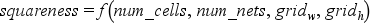
\includegraphics{./square_f.png}
        %    \caption{Squareness Function}
        %\end{figure}

        %\begin{figure}[H]
        %    \centering
        %    \includegraphics[width=\linewidth, height=2in, keepaspectratio]{../benchmarks/10_placement_0_start.jpg}
        %    \caption{Original}
        %\end{figure}
        %\begin{figure}[H]
        %    \centering
        %    \includegraphics[width=\linewidth, height=2in, keepaspectratio]{../benchmarks/10_placement_1_force.jpg}
        %    \caption{Force Directed}
        %\end{figure}


\newpage
\section{Usage}

Building is accomplished via a \texttt{Makefile} which generates an executable
names \texttt{main}. Additional build opions are shown below.

\begin{lstlisting}[language=bash]
$ make              # regular build
$ make clang        # builds using clang++ instead of g++
$ make debug        # enable debug printfs
$ make clean        # removes all binaries, object files, and benchmark results
$ make benchmarks   # runs all the benchmarks in the 'benchmark' directory
$ make pngs         # converts all the benchmark .svg files to .png
$ make jpgs         # converts all the .png files to reduced resolution .jpg files
\end{lstlisting}

The program accepts a single argument which is a file containing the netlist
formatted as specified in the assignment. All log and debug output is printed
to \texttt{stdout} and the output .mag and .svg files are named the same as the
input file.

\begin{lstlisting}[language=bash]
$ ./main benchmark/1 > benchmark/1.log
$ ls benchmark/1.*
benchmarks/1.log  benchmarks/1.mag benchmarks/1.svg
\end{lstlisting}

\section{Results}

    \subsubsection{Performance}
    \begin{table}[H]
        \centering
        \begin{tabular}{l|c|c|c|l}
            \toprule
            %\textbf{Benchmark} & \textbf{Tautology} & \textbf{Execution Time (s)} & \textbf{Memory} & \textbf{Algorithm Used} \\
            \specialcell{Benchmark} & \specialcell{Tautology} & \specialcell{Execution\\Time(s)} & \specialcell{Memory} & \specialcell{Algorithm\\Used} \\
            \midrule
            Cover1\_8\_10           & NO                      &                                  &                      & Heuristic Method \\
            Cover2\_8\_100          & NO                      &                                  &                      & Flags Method     \\
            Cover3\_8\_250          & YES                     &                                  &                      & Flags Method     \\
            Cover4\_15\_1000        & NO                      &                                  &                      & Heuristic Method \\
            Cover5\_15\_10000       & YES                     &                                  &                      & Flags Method     \\
            Cover6\_15\_30000       & YES                     &                                  &                      & Flags Method     \\
            Cover7\_20\_10000       & NO                      &                                  &                      & Heuristic Method \\
            Cover8\_20\_100000      & YES                     &                                  &                      & Flags Method     \\
            Cover9\_20\_1000000     & YES                     &                                  &                      & Flags Method     \\
            Cover\_25\_100000       & NO                      &                                  &                      & Heuristic Method \\
            Cover\_25\_1000000      & YES                     &                                  &                      & Flags Method     \\
            Cover\_25\_10000000     & YES                     &                                  &                      & Flags Method     \\
            Cover\_30\_1000000      & NO                      &                                  &                      & Heuristic Method \\
            Cover\_30\_10000000     &                         &                                  &                      & \\
            Cover\_30\_100000000    &                         &                                  &                      & \\
            \bottomrule
        \end{tabular}
        \caption{Execution time and memory for each run of cc and tc}
    \end{table}

    %probably just change everything so that we run each cover with both
    %programs because maybe it takes like 7 seconds to determine that
    %the cover is a tautology, but then again why do we have to
    %implement tc and cc if cc does both, i don't know...
    \textit{Note: If the cover was found to be not a tautology, the
        complement algorithm was run, therefore column two conveys whether
        cc or tc was run. For example, in Row 1, we see that the cover is
        not a tautology, therefore the execution time and memory used takes
        in account for both cc and tc, whereas for \texttt{Cover3\_8\_250},
        it was found to be a tautology so the data reflects only for the tc
        program.}

    %\begin{table}[H]
    %    \centering
    %    \begin{tabular}{ccccccccc}
    %        \toprule
    %        \textbf{Benchmark} &
    %        \specialcell{Box X} & \specialcell{Box Y} & \specialcell{Box Area} &
    %        \specialcell{\# FTs} & \specialcell{Wirelength} & \specialcell{\# Vias} &
    %        \specialcell{Execution Time} & \specialcell{Memory Usage}\\
    %        \midrule
    %        \phantom{0}1 & \phantom{00}82 & \phantom{00}76 & \phantom{000}6232 & \phantom{00}17 & \phantom{00}1093 & \phantom{0}112 & 0.009873s & \phantom{0}296 kB \\
    %        \phantom{0}2 & \phantom{0}127 & \phantom{0}129 & \phantom{00}16383 & \phantom{00}50 & \phantom{00}2547 & \phantom{0}270 & 0.021806s & \phantom{0}340 kB \\
    %        \phantom{0}3 & \phantom{0}191 & \phantom{0}175 & \phantom{00}33425 & \phantom{0}112 & \phantom{00}6114 & \phantom{0}562 & 0.044696s & \phantom{0}424 kB \\
    %        \phantom{0}4 & \phantom{0}317 & \phantom{0}252 & \phantom{00}79884 & \phantom{0}213 & \phantom{0}14108 & \phantom{}1126 & 0.111609s & \phantom{0}588 kB \\
    %        \phantom{0}5 & \phantom{0}486 & \phantom{0}403 & \phantom{0}195858 & \phantom{0}464 & \phantom{0}41469 & \phantom{}2336 & 0.384445s & \phantom{0}916 kB \\
    %        \phantom{0}6 & \phantom{0}602 & \phantom{0}513 & \phantom{0}308826 & \phantom{0}685 & \phantom{0}70536 & \phantom{}3322 & 0.670760s & \phantom{}1204 kB \\
    %        \phantom{0}7 & \phantom{}1110 & \phantom{}1130 & \phantom{}1254300 & \phantom{}1738 & \phantom{}443767 & \phantom{}5448 & 1.581445s & \phantom{}1512 kB \\
    %        \phantom{0}8 & \phantom{0}437 & \phantom{0}333 & \phantom{0}145521 & \phantom{0}297 & \phantom{0}22907 & \phantom{}1994 & 0.360278s & \phantom{0}912 kB \\
    %        \phantom{0}9 & \phantom{0}328 & \phantom{0}229 & \phantom{00}75112 & \phantom{00}69 & \phantom{00}6097 & \phantom{0}842 & 0.206668s & \phantom{0}664 kB \\
    %        \phantom{}10 & \phantom{0}258 & \phantom{0}202 & \phantom{00}52116 & \phantom{00}35 & \phantom{00}2881 & \phantom{0}404 & 0.157362s & \phantom{0}544 kB \\
    %        \bottomrule
    %    \end{tabular}
    %    \caption{Result Summary}
    %\end{table}

%%\for%each \i in {1,...,10} {
%    \newpage
%    \subsection{Benchmark \i\thinspace - Placement Steps}
%    \placementimage{../benchmarks/\i_placement_0_start.jpg}      {Benchmark \i\thinspace - Step 1/7 - Initial placement}
%    \placementimage{../benchmarks/\i_placement_1_force.jpg}      {Benchmark \i\thinspace - Step 2/7 - Force directed placement}
%    \placementimage{../benchmarks/\i_placement_2_flip.jpg}       {Benchmark \i\thinspace - Step 3/7 - Flip cells}
%    \placementimage{../benchmarks/\i_placement_3_feed.jpg}       {Benchmark \i\thinspace - Step 4/7 - Add feed-throughs}
%    \placementimage{../benchmarks/\i_placement_4_feed_even.jpg}  {Benchmark \i\thinspace - Step 5/7 - Even out the row length}
%    \placementimage{../benchmarks/\i_placement_5_pull.jpg}       {Benchmark \i\thinspace - Step 6/7 - Pull cells in the rows closer together}
%    \placementimage{../benchmarks/\i_placement_6_feed_moved.jpg} {Benchmark \i\thinspace - Step 7/7 - Move feed-throughs to optimal location}
%
%    \newpage
%    \subsection{Benchmark \i\thinspace - Final Routing}
%    \begin{figure}[H]
%        \centering
%        \includegraphics[width=\linewidth]{../benchmarks/\i.jpg}
%        \caption{Benchmark \i\thinspace - Final routing}
%    \end{figure}
%
%    \newpage
%    \subsection{Benchmark \i\thinspace - Magic Screenshot}
%    \begin{figure}[H]
%        \centering
%        \includegraphics[width=\linewidth]{./magic_\i.png}
%        \caption{Benchmark \i\thinspace - Magic Screenshot}
%    \end{figure}
%
%    \newpage
%    \subsection{Benchmark \i\thinspace - Log file}
%    \lstinputlisting[caption=Benchmark \i\thinspace - Log]{../benchmarks/\i.log}
%}

\newpage
%Include a retrospective describing what you think is the cause of the good/poor performance of your
%tools and how might you be able to improve the performance if you had more time?
\section{Retrospective}

Overall, we are pretty satisfied with both the execution speed and quality of
our results. All of our execution times with the exception of benchmark 7 are
under half a second. We also feel that our memory usage is minimal as we only
store one vector of actual cell objects and all other data structures just
contain pointers back to the original objects. We also make heavy use of pass
by reference to avoid needlessly copying big data structures into functions.

In terms of placement and routing quality there is always room for improvement.
It's easy to visually look at almost any result and see ways that it could be
improved but how to translate these improvements into algorithms is not always
so obvious. We believe, however, that we were are able to handle a lot of
specific cases (like moving the feed-throughs to the other side of the cell)
which in the end resulted in superior layouts.  For the force directed
placement algorithm it is hard to tell if the results you get are truly the
best, especially when the circuit is so large you cannot visually comprehend
it. We feel like we did our best analyzing it empirically and tuned is to best
suit our benchmark files. One of the main problems with the force directed
algorithm is that it tends to pull all the cells into the center of the layout.
We tried to fix this by redistributing the unconnected cells evenly through the
layout and then re-force directing the rows but it is still not always ideal.
One interesting method to pursue would be using a combination of min-cut /
quadratic placement and then force directing the sub divisions (or vice versa).
If we were to min-cut horizontally we might be able to reduce some nets that
currently span multiple rows.


\newpage
\section{Appendix}

\end{document}
